\documentclass[aspectratio=169]{../latex_main/tntbeamer}  % you can pass all options of the beamer class, e.g., 'handout' or 'aspectratio=43'
\usepackage{dsfont}
\usepackage{bm}
\usepackage[english]{babel}
\usepackage[T1]{fontenc}
%\usepackage[utf8]{inputenc}
\usepackage{graphicx}
\graphicspath{ {./figures/} }
\usepackage{algorithm}
\usepackage[ruled,vlined,algo2e,linesnumbered]{algorithm2e}
\usepackage{hyperref}
\usepackage{booktabs}
\usepackage{mathtools}

\usepackage{amsmath,amssymb}

\DeclareMathOperator*{\argmax}{arg\,max}
\DeclareMathOperator*{\argmin}{arg\,min}

\usepackage{amsbsy}
\newcommand{\vect}[1]{\bm{#1}}
%\newcommand{\vect}[1]{\boldsymbol{#1}}

\usepackage{pgfplots}
\pgfplotsset{compat=1.16}
\usepackage{tikz}
\usetikzlibrary{trees} 
\usetikzlibrary{shapes.geometric}
\usetikzlibrary{positioning,shapes,shadows,arrows,calc,mindmap}
\usetikzlibrary{positioning,fadings,through}
\usetikzlibrary{decorations.pathreplacing}
\usetikzlibrary{intersections}
\pgfdeclarelayer{background}
\pgfdeclarelayer{foreground}
\pgfsetlayers{background,main,foreground}
\tikzstyle{activity}=[rectangle, draw=black, rounded corners, text centered, text width=8em]
\tikzstyle{data}=[rectangle, draw=black, text centered, text width=8em]
\tikzstyle{myarrow}=[->, thick, draw=black]

% Define the layers to draw the diagram
\pgfdeclarelayer{background}
\pgfdeclarelayer{foreground}
\pgfsetlayers{background,main,foreground}

% Requires XeLaTeX or LuaLaTeX
%\usepackage{unicode-math}

\usepackage{fontspec}
%\setsansfont{Arial}
\setsansfont{RotisSansSerifStd}[ 
Path=../latex_main/fonts/,
Extension = .otf,
UprightFont = *-Regular,  % or *-Light
BoldFont = *-ExtraBold,  % or *-Bold
ItalicFont = *-Italic
]
\setmonofont{Cascadia Mono}[
Scale=0.8
]

\renewcommand{\ttdefault}{Cascadia Mono}

% scale factor adapted; mathrm font added (Benjamin Spitschan @TNT, 2021-06-01)
%\setmathfont[Scale=1.05]{Libertinus Math}
%\setmathrm[Scale=1.05]{Libertinus Math}

% other available math fonts are (not exhaustive)
% Latin Modern Math
% XITS Math
% Libertinus Math
% Asana Math
% Fira Math
% TeX Gyre Pagella Math
% TeX Gyre Bonum Math
% TeX Gyre Schola Math
% TeX Gyre Termes Math

% Literature References
\newcommand{\lit}[2]{\href{#2}{\footnotesize\color{black!60}[#1]}}

%%% Beamer Customization
%----------------------------------------------------------------------
% (Don't) Show sections in frame header. Options: 'sections', 'sections light', empty
\setbeamertemplate{headline}{empty}

% Add header logo for normal frames
\setheaderimage{
	% 
\includegraphics[height=\logoheight]{figures/TNT_darkv4.pdf}
	
\includegraphics[height=\logoheight]{../latex_main/figures/Leibniz-AI-Academy_Logo}
	% 
\includegraphics[height=\logoheight]{figures/logo_tntluh.pdf}
}

% Header logo for title page
\settitleheaderimage{
	% 
\includegraphics[height=\logoheight]{figures/TNT_darkv4.pdf}
	
\includegraphics[height=\logoheight]{../latex_main/figures/Leibniz-AI-Academy_Logo}
	% 
\includegraphics[height=\logoheight]{figures/logo_tntluh.pdf}
}

% Title page: tntdefault 
\setbeamertemplate{title page}[tntdefault]  % or luhstyle
% Add optional title image here
%\addtitlepageimagedefault{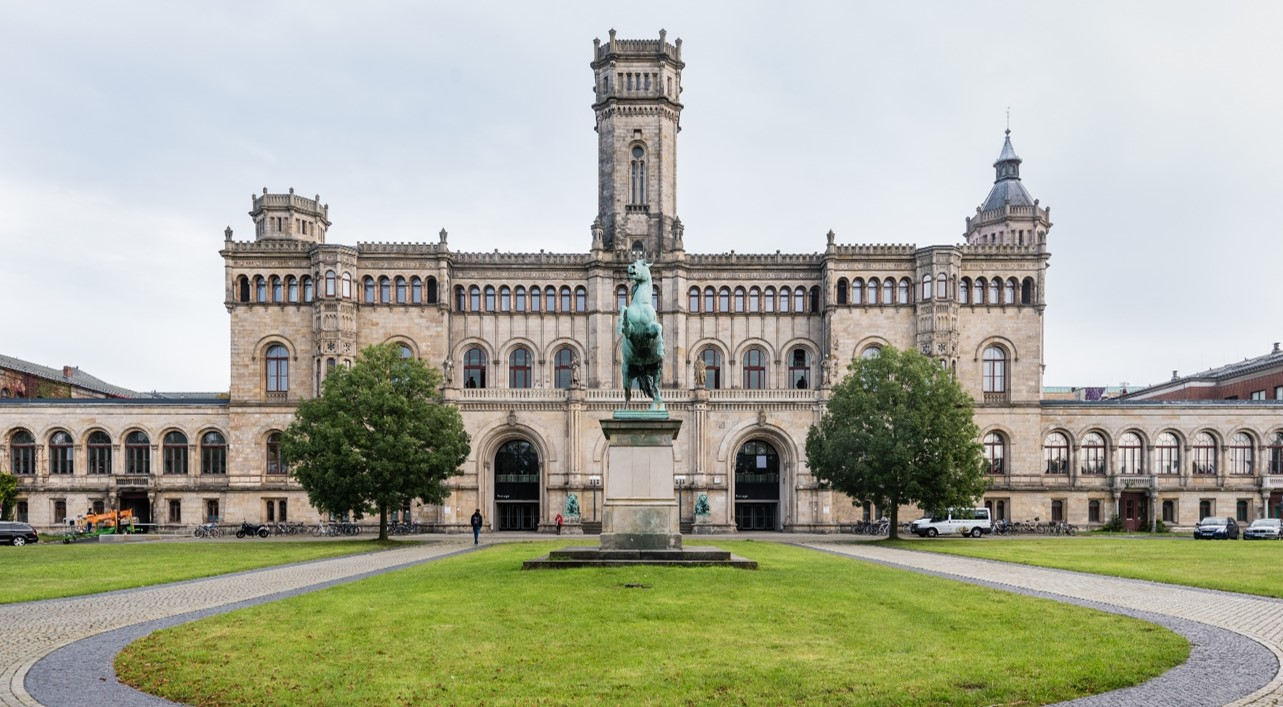
\includegraphics[width=0.65\textwidth]{figures/luh_default_presentation_title_image.jpg}}

% Title page: luhstyle
% \setbeamertemplate{title page}[luhstyle]
% % Add optional title image here
% \addtitlepageimage{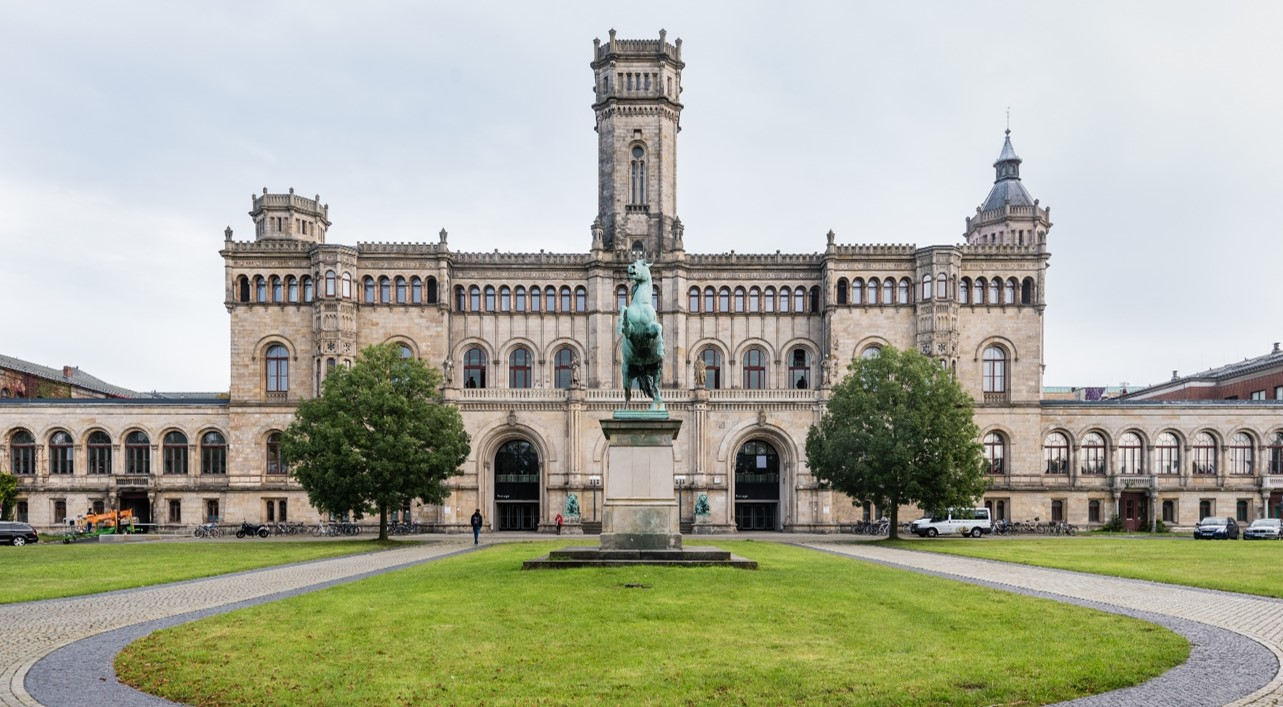
\includegraphics[width=0.75\textwidth]{figures/luh_default_presentation_title_image.jpg}}

\author[Abedjan \& Lindauer]{Ziawasch Abedjan \& \underline{Marius Lindauer}\\[1em]
	%
\includegraphics[height=\logoheight]{../latex_main/figures/luh_logo_rgb_0_80_155.pdf}\qquad
	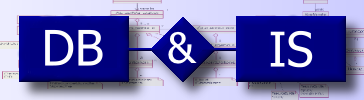
\includegraphics[height=\logoheight]{../latex_main/figures/DBIS_Kurzlogo.png}\qquad
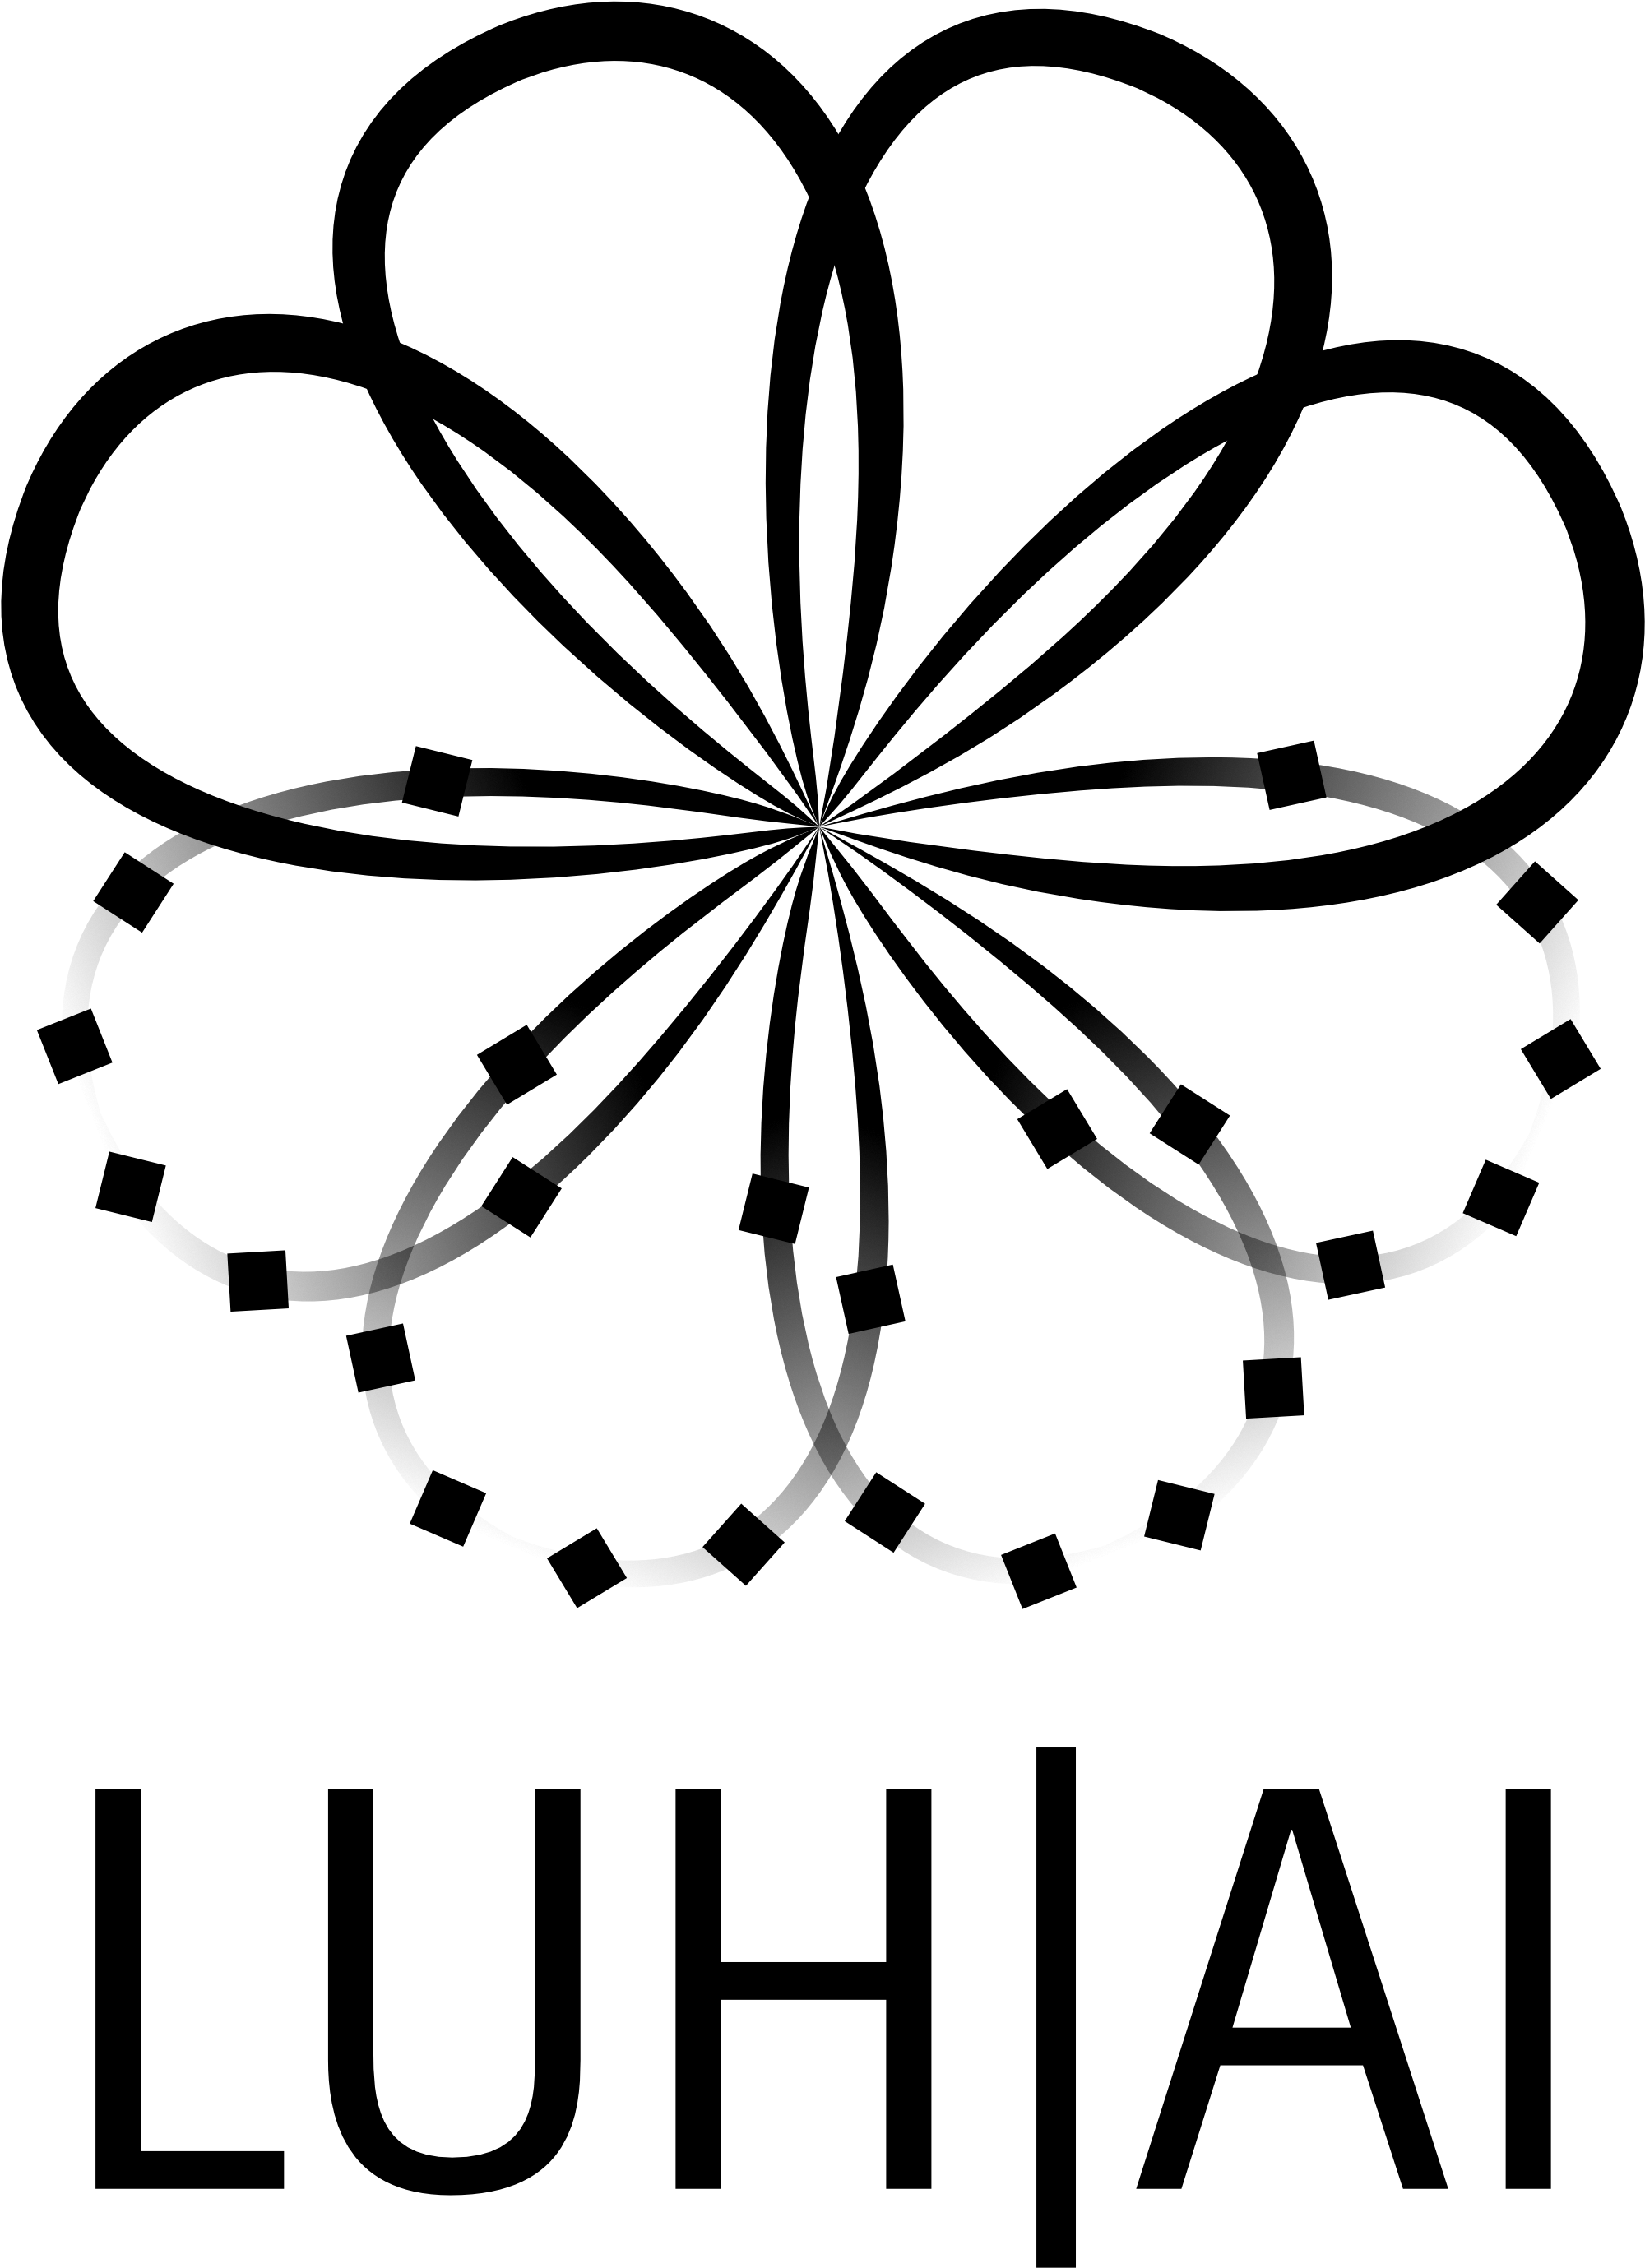
\includegraphics[height=\logoheight]{../latex_main/figures/logo_short_highres_black}\qquad

\includegraphics[height=\logoheight]{../latex_main/figures/Leibniz-AI-Academy_Logo}\qquad
%
\includegraphics[height=\logoheight]{../latex_main/figures/L3S.jpg}	
}
\date{\hspace{0.5em} {
\includegraphics[height=1.5em]{../latex_main/figures/Cc-by-nc-sa_icon.svg.png}}; extension of \href{https://ds100.org/fa21/}{[DS100]}
}


%%% Custom Packages
%----------------------------------------------------------------------
% Create dummy content
\usepackage{blindtext}

% Adds a frame with the current page layout. Just call \layout inside of a frame.
\usepackage{layout}


%%% Macros
%\renewcommand{\vec}[1]{\mathbf{#1}}
% \usepackage{bm}
%\let\vecb\bm

\title[DL in a Nutshell]{DS: Deep Learning}
\subtitle{DL in a Nutshell}

\date{\hspace{0.5em} {
\includegraphics[height=1.5em]{../latex_main/figures/Cc-by-nc-sa_icon.svg.png}}; Inspired by \href{https://www.deeplearning.ai/resources/}{Andrew Ng}}

\graphicspath{ {./figure/} }
%\institute{}


\begin{document}
	
	\maketitle
	\begin{frame}{Scaling with Data}

        \begin{itemize}
            \item More and more data is available these days
            \begin{itemize}
                \item with all its benefits and downsides
            \end{itemize}
            \item Models need to scale with data
        \end{itemize}

        \centering
        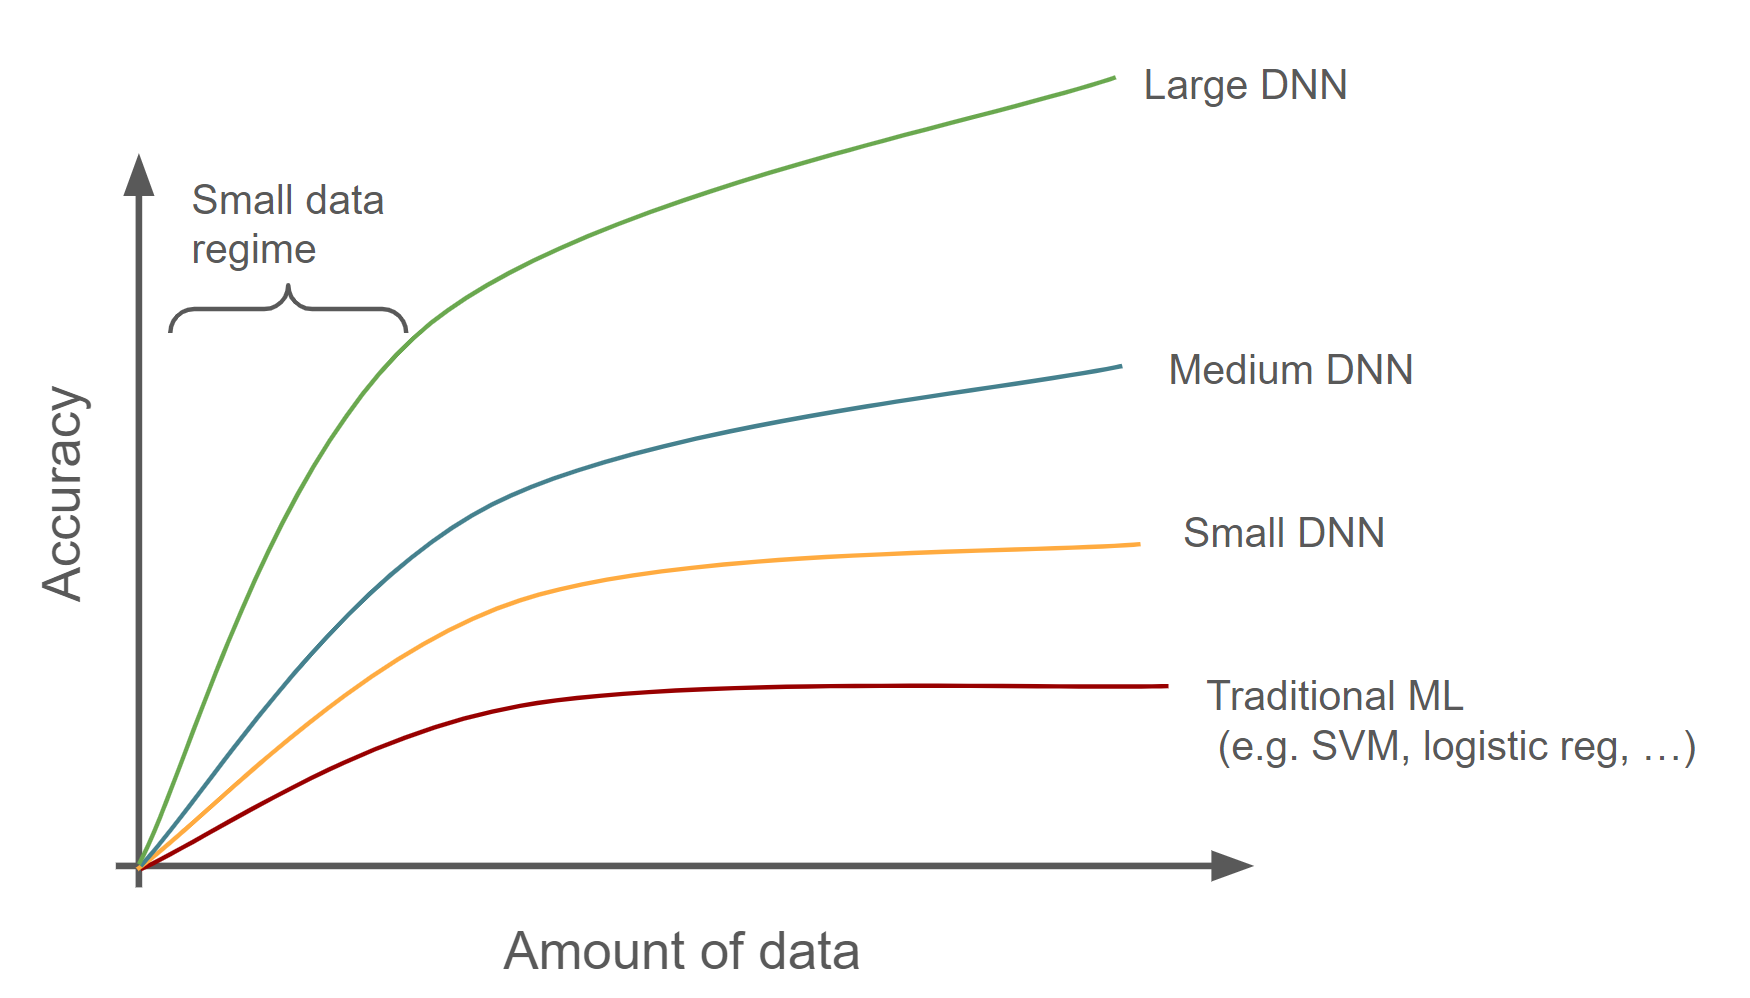
\includegraphics[width=0.6\textwidth]{figure/dl_scaling}


	\end{frame}

 	\begin{frame}{Layer-wise Feature Engineering}
        % Housing Price Prediction

        \begin{itemize}
            \item By combining features, you can get interesting new features
            \item Main idea: combine features (pairwise) in each layer and build stronger and stronger feature representations
            \item Important: A linear combination of a linear combination of features is still a linear combination $\leadsto$ we need non-linear combinations
        \end{itemize}

        \centering
        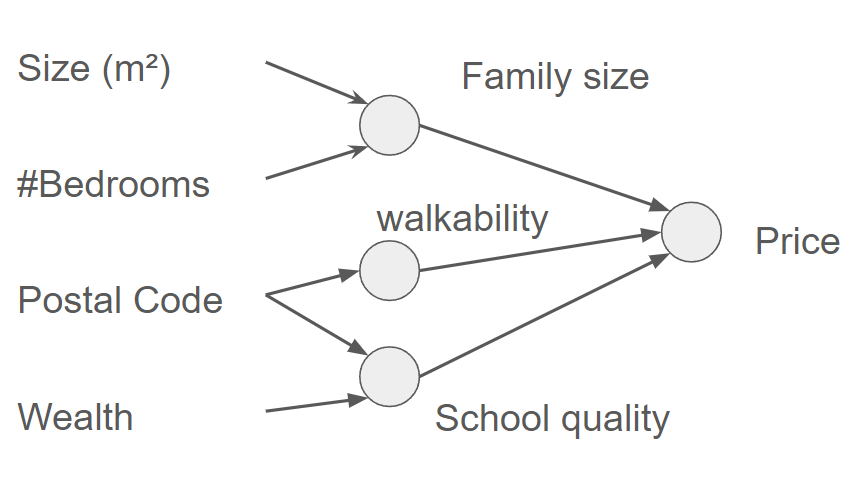
\includegraphics[width=0.4\textwidth]{figure/layer_rep}

	\end{frame}

  	\begin{frame}{Application to different Tasks and Data Modalities}
        % table Input, Output, Application, Modality, Network Type

        {\centering
        \begin{tabular}{lllll}
             Input & Output & Application & Modality & Network Type  \\
             \midrule
             Home Features & Price & Real Estate & Table & MLP \\ \pause
             Ad, user info & Click on ad? (binary) & Online Advertising & Table & MLP\\ \pause
             Image & Object (1,\ldots, 1000) & Photo Tagging & Images & CNN\\ \pause
             Audio & Text transcript & Speech recognition & Audio Sequence & RNN\\ \pause
             English & German & Machine Translation & Text & Transformer\\ \pause
             Image, Radar Info & Position of other cars & Autonomous driving & Multi-modal & Custom\\ \pause
        \end{tabular}}

        \vspace{2em}

        $\leadsto$ Consider input, output and data modality to decide which kind of network type you need\\ -- more details later!

	\end{frame}
	

   	\begin{frame}{Structured vs Unstructured Data}
        % Structured Data: Table
        % Unstructured Data: Image, Audio, Text

        \begin{columns}

        \column{0.5\textwidth}

        Structure data: Tables\\[2em]

        \centering
        \begin{tabular}{llc|r}
             Size & bedrooms & \ldots & Price  \\
             \midrule
             2104 & 3       & & 400.000\\
             1600 & 3 & & 330.000\\
             \ldots \\
             3000 & 4 & & 540.000\\
        \end{tabular}

        \column{0.5\textwidth}
            
        
        
        Unstructured Data

        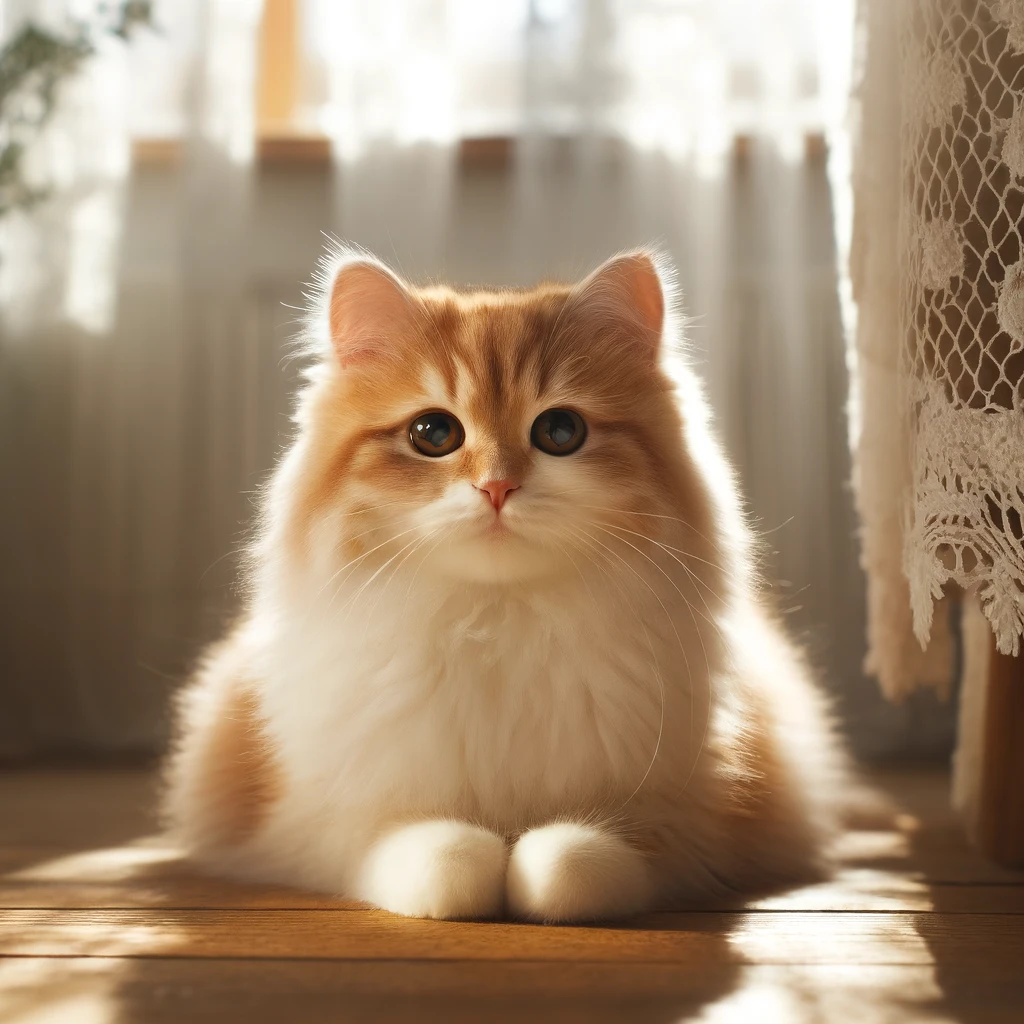
\includegraphics[width=0.4\textwidth]{figure/cat.png}
        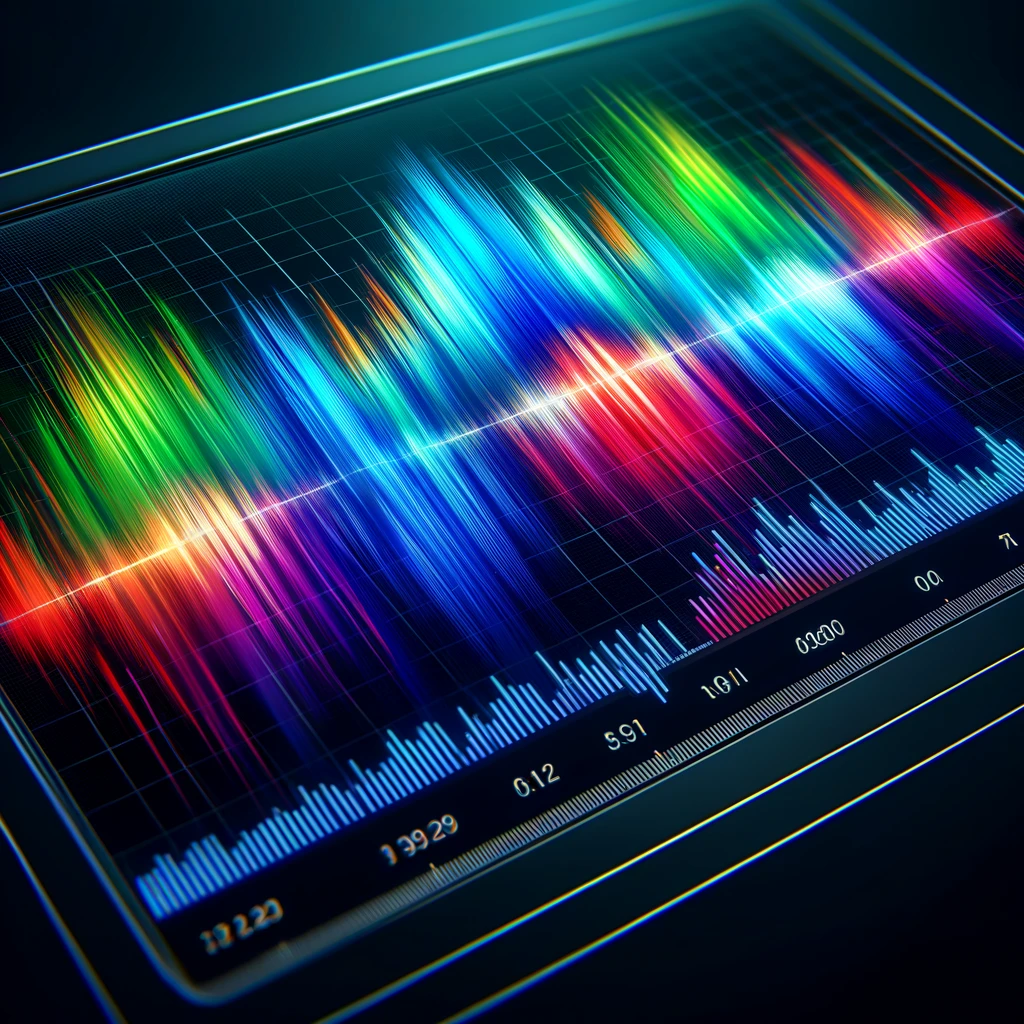
\includegraphics[width=0.4\textwidth]{figure/audio.png}

        \vspace{2em}

        Text: \textit{Once upon a time, there was \ldots}

        \end{columns}

        $\leadsto$ So far, Deep Learning is mostly successful on unstructured data (e.g., images, sound, text). 

	\end{frame}

\end{document}